\documentclass{jsarticle}

 \usepackage{ascmac}
 \usepackage{graphicx}
 \usepackage[dvipdfmx]{color}
 \usepackage{amssymb,amsmath,amsthm}
 \usepackage{graphics}
 \usepackage{fancybox, tcolorbox}
 \tcbuselibrary{raster,skins, breakable}
 \usepackage{nccmath}
 \usepackage{tikz}
 \usetikzlibrary{intersections, calc, cd}
 \usepackage{bm}
 \usepackage[italicdiff]{physics}
 \usepackage{titlesec}
 \usepackage{mathtools}
 \usepackage{enumerate}
 \usepackage{float}


 \newcommand{\myproof}[1]{
  \begin{tcolorbox}[
    empty,top = -2pt, breakable = true,
    underlay = {
      \draw[line width = 5pt, color = teal] (frame.north west) -- (frame.south west);
      },
    underlay unbroken = {
      \fill (frame.south east) -- ([xshift = -5pt]frame.south east) --([xshift = -5pt, yshift = -7pt]frame.south east) -- ([yshift = -7pt]frame.south east) -- cycle;
    },
    underlay last = {
        \fill (frame.south east) -- ([xshift = -5pt]frame.south east) --([xshift = -5pt, yshift = -7pt]frame.south east) -- ([yshift = -7pt]frame.south east) -- cycle;
      }
    ]
    {\it Proof.}

    {#1}
  \end{tcolorbox}
 }

 \setcounter{tocdepth}{3}

\theoremstyle{definition}
\newtheorem{dfn}{定義}[section]
\newtheorem{exa}{例}[section]
\newtheorem{thm}[dfn]{定理}
\newtheorem{prop}[dfn]{命題}
\newtheorem{note}[dfn]{注意}
\newtheorem{prob}[dfn]{問}
\newtheorem{coro}[dfn]{系}


\title{}
\author{八木俊輔}
\date{\today}

\usepackage{fancyhdr}
\pagestyle{fancy}
    \lfoot{}
    \cfoot{\thepage}
    \rfoot{}

\begin{document}
ここでは文献[1]と同じモデルを考える.
\begin{figure}[H]
  \begin{center}
  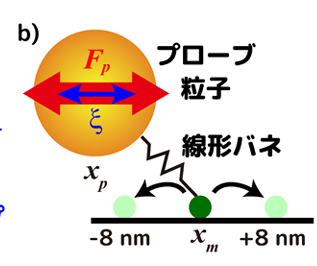
\includegraphics[width=5cm]{kinesin.png}
  \end{center}
  \caption{kinesinのモデル}
\end{figure}
このモデルでのLangevin方程式は
\begin{equation}
  \gamma \dot{x}_p(t) = k (x_m (t) - x_p(t)) + F_0 + F_n (t) + \eta(t)
\end{equation}
となる.ここで $\gamma, k$ は粘性抵抗,ばね定数である.
$x_p(t), x_m (t)$はプローブ,キネシンの位置であり,$F_0$は一定の外力,$F_n (t)$は平均 $0$ のゆらぐ力,$\eta (t)$は白色ガウス型の熱ゆらぎである.
ただし,熱ゆらぎはつぎを満たすものとする.
\begin{equation}
  \langle \eta (t) \eta (s) \rangle = 2 k_B T \gamma \delta (t-s)
\end{equation}
また,ゆらぐ力はラビィ型の分布を示すことが知られており,その分散は無限大の大きさを持つが,ここでは定数 $f$ を用いて
\begin{equation}
  \langle F_n (t) F_n (s) \rangle = 2 f \delta (t-s)
\end{equation}
という関係を満たすようにしておく.これは実験では技術的な制約により,その大きさは有限の値になっていたためである.\\
\quad ここで測定ができる文字は 
\begin{equation}
  \gamma, x_p (t), k, F_0
\end{equation}
の4つであり,$x_m (t)$ の測定はできないことに注意して,VSRを考える.\\

[1] Ariga, Takayuki, et al. "Noise-induced acceleration of single molecule kinesin-1." Physical review letters 127.17 (2021): 178101.

\end{document}